% Section content template for individual Educative lessons
% This file contains the actual content for a specific section
% Generated from Educative API section content

% Section: System Design: The Content Delivery Network (CDN)
% Section ID: 6624266925899776
% Section Slug: system-design-the-content-delivery-network-cdn
% Generated: 2025-12-07T17:12:52.410174

\subsection{Problem statement}\label{268AxlhCVaeYijWg8uJkv}
\\
Let's start with a question: If millions of users worldwide use our data-intensive applications, and our service is deployed in a single data center to serve the users' requests, what possible problems can arise?
\\
The following problems can arise:

\begin{itemize}
\item
\protect\phantomsection\label{qxytN-J77Key7tzaA0yBK}
\textbf{High latency}: The user-perceived latency will be high due to the physical distance from the serving data center. User-perceived latency has many components, such as transmission delays (a function of available bandwidth), propagation delays (a function of distance), queuing delays (a function of network congestion), and nodal processing delays. Therefore, data transmission over a large distance results in higher latency. Real-time applications require a latency below 200 milliseconds (ms) in general. For the Voice over Internet Protocol (VoIP), latency should not be more than 150 ms, whereas video streaming applications cannot tolerate a latency above a few seconds.
\end{itemize}
\begin{quote}
\textbf{Note:} According to one of the readings taken on December 21, 2021, the average latency from US East (N. Virginia) to US West (N. California) was 62.9 ms. Across continents---for example, from the US East (N. Virginia) to Africa (Cape Town)---was 225.63 ms. This is two-way latency, known as round-trip latency.
\end{quote}

\begin{figure}[htbp]
 \centering
 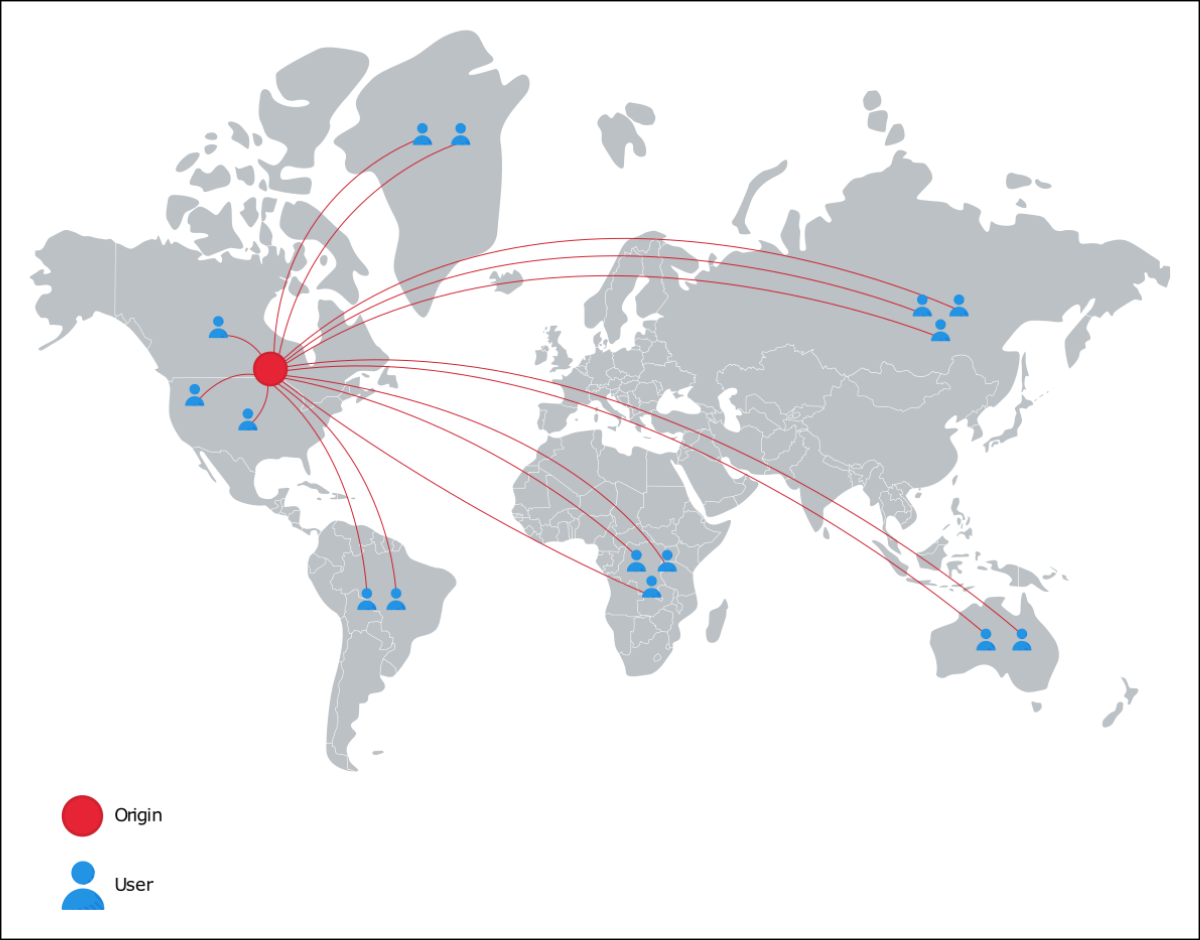
\includegraphics[width=0.5\textwidth]{Images/chapter_11/section_6624266925899776/4856140645400576.png}
 \caption{Origin data center entertaining users' requests across the globe}
\end{figure}

\begin{itemize}
\item
\protect\phantomsection\label{G_MapmNtWcGMEvH-p2D9F}
\textbf{Data-intensive applications}: Data-intensive applications require transferring large traffic. Over a longer distance, this could be a problem due to the network path stretching through different kinds of ISPs. Because of some smaller Path message transmission unit(A Path MTU refers to the largest data unit that can traverse from source to destination without the need for splitting.) (MTU) links, the throughput of applications on the network might be reduced. Similarly, different portions of the network path might have different congestion characteristics. The problem multiplies as the number of users grows because the origin servers will have to provide the data individually to each user. That is, the primary data center will need to send out a lot of redundant data when multiple clients ask for it. However, applications that use streaming services are both data-intensive and dynamic in nature.
\end{itemize}
\begin{quote}
\textbf{Note:} According to a survey(These statistics represent the number of shares, in the US from 2015 to 2021, of those consumers who have a subscription video-on-demand (SVOD).), 78\% of the United States consumers use streaming services, which is an increase of 25\% in five years.
\end{quote}
\begin{itemize}
\item
\protect\phantomsection\label{FOqxnKBlUk3roTEpSlkwi}
\textbf{Scarcity of data center resources}: Important data center resources like computational capacity and bandwidth become a limitation when the number of users of a service increases significantly. Services engaging millions of users simultaneously need scaling. Even if scaling is achieved in a single data center, it can still suffer from becoming a single point of failure when the data center goes offline due to natural calamity or connectivity issues with the Internet.
\end{itemize}

\begin{figure}[htbp]
 \centering
 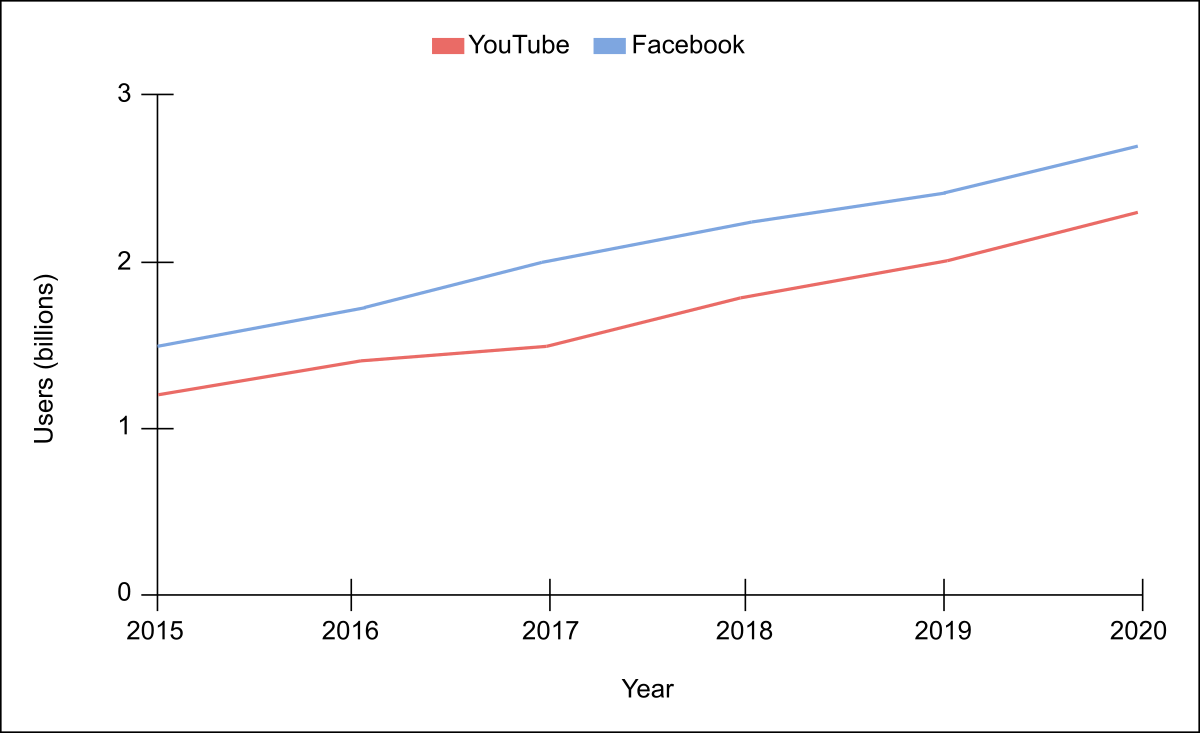
\includegraphics[width=0.5\textwidth]{Images/chapter_11/section_6624266925899776/4758001179557888.png}
 \caption{User growth over the years for Facebook and YouTube applications}
\end{figure}

\begin{quote}
\textbf{Note:} According to one study, YouTube, Netflix, and Amazon Prime collectively generated 80\% of Internet traffic in 2020. Circa 2016, the CDN provider Akamai served 15\% to 30\% of web traffic (about 30 terabits per second). For 90\% of Internet users, Akamai was just one hop away. Therefore, we have strong reasons to optimize the delivery and consumption of this data without making the Internet core a bottleneck.
\end{quote}
\\
The solution to these problems is a content delivery network (CDN), a system that brings data closer to users around the world.

\subsection{How will we design a CDN?}\label{jYuXRdmFv1MxED915XUYp}
\\
We've divided the design of CDN into six lessons:

\begin{enumerate}
\item
\protect\phantomsection\label{-335yulP0aW3neEBXEvSQ}
\href{https://www.educative.io/courses/grokking-the-system-design-interview/introduction-to-a-cdn}{\textbf{Introduction to a CDN}}: We'll provide a thorough introduction to CDNs and identify the functional and non-functional requirements.
\item
\protect\phantomsection\label{kn-XQrdzdFCAg85OVQ32q}
\href{https://www.educative.io/courses/grokking-the-system-design-interview/design-of-a-cdn}{\textbf{Design of a CDN}}: We'll explain how to design the CDN. We'll also briefly describe the API design.
\item
\protect\phantomsection\label{6mROXyrpTmP6rmXpfUdPo}
\href{https://www.educative.io/courses/grokking-the-system-design-interview/in-depth-investigation-of-cdn-part-1}{\textbf{In-depth Investigation of CDN: Part 1}}: This lesson explains caching strategies and CDN architecture. Also, we'll discuss various approaches to finding the nearest proxy server.
\item
\protect\phantomsection\label{ThftFzMZtYtlM8h5Ih_rL}
\href{https://www.educative.io/courses/grokking-the-system-design-interview/in-depth-investigation-of-cdn-part-2}{\textbf{In-depth Investigation of CDN: Part 2}}: We'll discuss how to make content consistent in a CDN and the deployment of proxy servers. We'll also cover the custom and specialized CDN in detail.
\item
\protect\phantomsection\label{lkUa_FuYs3w9EWtp6KcYE}
\href{https://www.educative.io/courses/grokking-the-system-design-interview/evaluation-of-cdns-design}{\textbf{Evaluation of CDN}}: This lesson will provide an evaluation of our proposed design.
\item
\protect\phantomsection\label{ZaesprjV9IXSYbm-w18q_}
\href{https://www.educative.io/courses/grokking-the-system-design-interview/quiz-on-cdns-design}{\textbf{Quiz on CDN System Design}}: We'll reinforce major concepts of CDN design with a quiz.
\end{enumerate}
\\
Let's begin!

% End of section content